\documentclass[pdf]
{beamer}
\mode<presentation>{}

\usepackage{amsmath}
\usepackage{tikz}
\usetikzlibrary{calc}                   
   

\newcommand\bayeseq{\mathrel{\overset{\makebox[0pt]{\mbox{\normalfont\tiny\sffamily Bayes}}}{=}}}

%% preamble
\title{Prediction of RNA and DNA binding sites: preliminary presentation}
\subtitle{}
\author[shortname]{Quirin Heiss\inst{1, 2} \and Pandu Raharja \inst{1, 2} \and Julian Schmidt \inst{1, 2}}
\institute[shortinst]{\inst{1} Technische Universit\"at M\"unchen \and %
                      \inst{2} Ludwig-Maximilians-Universit\"at M\"unchen}
\begin{document}

%% title frame
\begin{frame}
\titlepage
\end{frame}

%% normal frame
\begin{frame}{Outline}
	\begin{itemize}
		\item Binding prediction and CAFA.
		\item Background: RNA and RNA binding proteins.
		\item Background: datasets.
		\item Steps    
	\end{itemize}
\end{frame}

\begin{frame}{Definition}
	\begin{itemize}
		\item \textbf{RNA/DNA Binding Protein prediction}: given a protein, determine whether a protein is RNA/DNA binding.
		\item \textbf{RNA/DNA binding site prediction}: given a protein sequence, determine side chains that bind with a DNA/RNA.
	\end{itemize}
\end{frame}

\begin{frame}{CAFA}
	\begin{enumerate}
		\item Determine whether protein is RNA or DNA binding.
		\item Determine binding site.
	\end{enumerate}
\end{frame}

\begin{frame}{Methods: abstraction level}
	\begin{figure}[ht]
		\begin{center}
			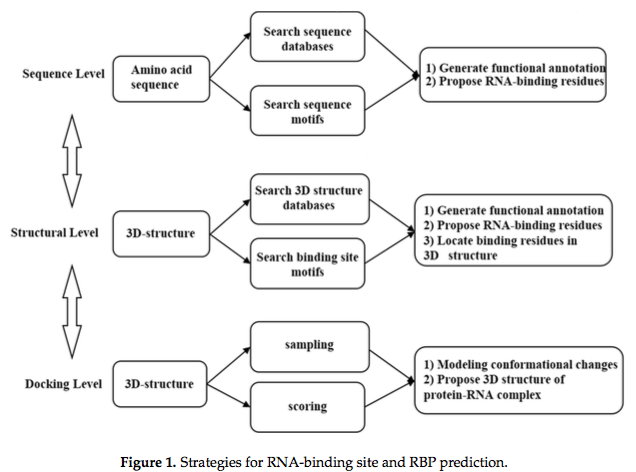
\includegraphics[height=2.5in]{ss_1.png}
			~\footnote{Si, Wu \textit{et al.}, 2015, \textit{Int. J. Mol. Sci.}}
		\end{center}
	\end{figure}
\end{frame}

\begin{frame}{Possible Features}
	Sequence-based features:
	\begin{itemize}
		\item \textbf{Amino acid composition}.
		\item \textbf{Sequence similarity,} such as MSA.
		\item \textbf{Evolutionary invormation,} such as PSSM. 
		\item \textbf{Evolutionary invormation,} such as PSSM. 
	\end{itemize}
	Structure-based features:
	\begin{itemize}
		\item \textbf{Secondary structure:} experimental (assigned using DSSPcont) or predicted.
		\item \textbf{Accessible surface area,} in percnent (\%).
	\end{itemize}
	Chemical and physical features:
	\begin{itemize}
		\item \textbf{Hydrophobicity.}
		\item \textbf{Electrostatic patches.}
		\item \textbf{Cleft Size.}
	\end{itemize}
\end{frame}

\begin{frame}{Methods: previously used algorithm}
	\begin{itemize}
		\item \textbf{Naive Bayes (NB)} classifier.
		\item \textbf{Support Vector Machine (SVM)}.
		\item \textbf{Random Forest}.
		\item \textbf{Neural Network (NN)}.
	\end{itemize}
	
	We think would be better:
	\begin{itemize}
		\item \textbf{Ensemble Learning}.
	\end{itemize}	
	
\end{frame}

\begin{frame}{Statistics}
	\begin{center}
		\begin{tabular}{| c | c |}
			\hline
			Name & Num\\
			\hline
			SwissProt (\texttt{HUMAN}) & 20120\\
			\texttt{GO:0003676} (\texttt{HUMAN}) & 1248\\
			SwissProt (filtered out \texttt{GO:0003676}) & 20005 \\
			\hline
		\end{tabular}	
	\end{center}
\end{frame}
	
\begin{frame}{Statistics (cont.)}

	Results of redundancy reduction on training set:\\
	\begin{center}
		\begin{tabular}{| c | c |}
			\hline
			Before & After\\
			\hline
			706 & 567\\
			\hline
		\end{tabular}		
	\end{center}
	
\end{frame}

\begin{frame}{Steps}

	\begin{itemize}
		\item Data pre-processing.
		\item Models development.
		\item Training.
		\item Validation.
	\end{itemize}
\end{frame}

\end{document}
